\chapter{Análisis de resultados}

En este capítulo se presenta el análisis y discusión de los principales resultados 
obtenidos en el desarrollo de este proyecto. Del análisis por elementos finitos 
se presentan los resultados del caso bidimensional y del modelo tridimensional, comparando 
ambos casos, con la finalidad de discutir la viabilidad de utilizar un análisis de tipo 
deformación plana en una simulación de formado como esta. Además los resultados del 
análisis numérico se comparan con lo obtenido mediante el análisis experimental.\\

Además, con la finalidad de determinar algunas condiciones o parámetros que faciliten 
el análisis de procesos de formado de este tipo, se presenta una sección destinada 
a evaluar la influencia del escalamiento de masa selectivo cuya utilidad va en 
dirección de disminuir el tiempo de cómputo requerido. Asimismo se expone una sección 
referente al uso de algunos modelos de material como el bilineal isotrópico y cinemático, 
la plasticidad cinemática y curvas multilineales, para determinar si las variaciones 
en el comportamiento del material son significativas.

\section{Del análisis de elementos finitos}

\subsection{Análisis 2D}

\subsubsection{Estatus global}

Normalmente en un análisis de tipo dinámico explícito, el balance de energía juega 
un papel importante e incluso puede utilizarse como criterio de \textit{terminación}. 
Para considerar que un análisis es aceptable, la energía cinética debe representar 
menos de un 5 \% de la energía interna del modelo, de lo contrario, los efectos 
inerciales inducidos podrían afectar de manera considerable tanto la geometría 
resultante como los datos de salida. En la figura \ref{fig:energy_status_01} se observa 
que la energía cinética representa un porcentaje menor al 1\% de la energía interna, lo 
cual implica que el análisis está dentro del rango aceptable. \\

\begin{center}
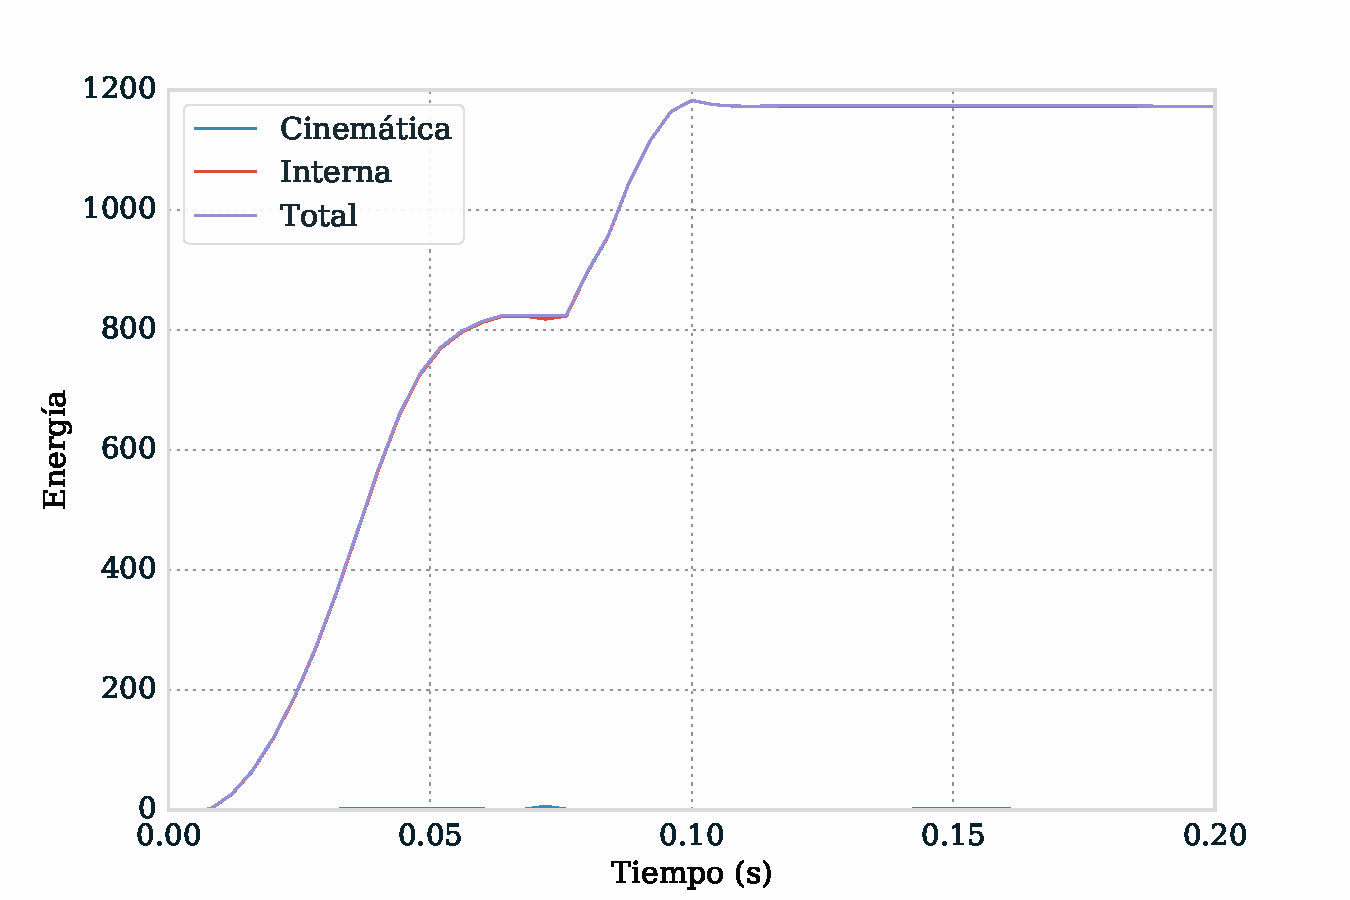
\includegraphics[width=0.8\textwidth]{src/ch4/energy_status_01.pdf}
\captionof{figure}{Variación de la energía total, interna y cinemática, primer paso}
\label{fig:energy_status_01}
\end{center}

El elemento \texttt{PLANE162}, utilizado en el mallado para el análisis bidimensional, 
tiene sólo un punto de integración, lo cual le hace robusto para grandes deformaciones 
y permite un ahorro significativo de tiempo computacional, pero esto mismo les hace 
propensos a presentar modos de energía cero. Estos modos, comúnmente referidos como 
modos de Hourglass, son de naturaleza oscilatoria y tienen periodos mucho más pequeños 
que la respuesta estructural de un sistema, resultando en estados matemáticos que físicamente 
no son posibles y que normalmente tienden a deformar la malla en forma de zigzag.
Para verificar que la deformación de Hourglass no ha influido de manera considerable 
en un análisis se debe comparar la energía interna del modelo con la energía de Hourglass, 
esta última no debe ser mayor al 10\% de la primera para considerar aceptable los 
resultados de la simulación ~\cite{lsdyna-ansys-manual}. En la gráfica de la figura \ref{fig:hourglass_internal_01} 
se muestra la energía interna vs la energía de Hourglass y se aprecia que la proporción 
varía en un rango del 1.5 a 2\%, lo cual indica que la deformación de Hourglass se encuentra 
dentro de los límites aceptables.


\begin{center}
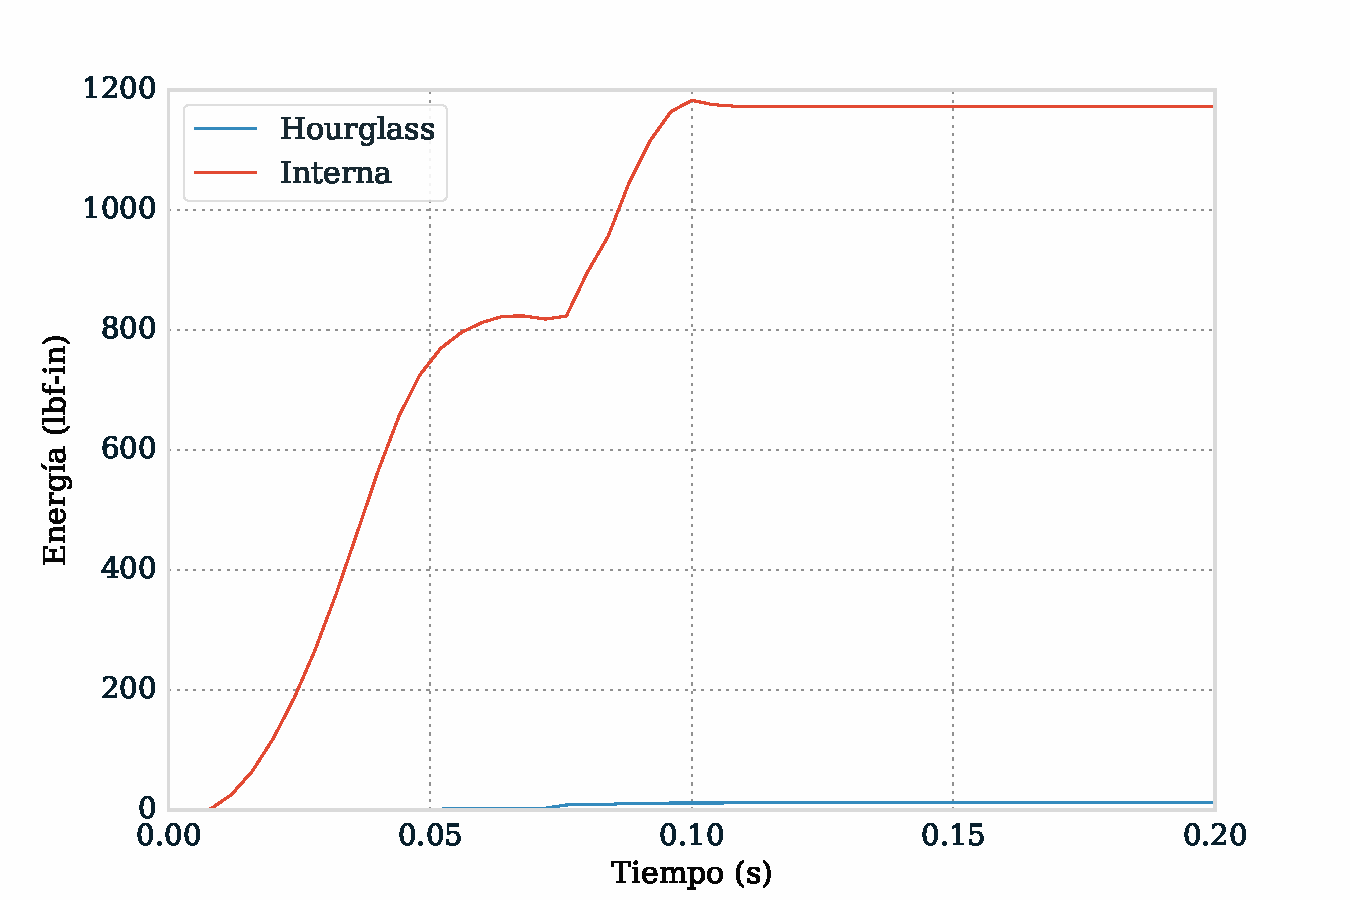
\includegraphics[width=0.8\textwidth]{src/ch4/hourglass_internal_01.pdf}
\captionof{figure}{Comparación energía interna vs energía de Hourglass}
\label{fig:hourglass_internal_01}
\end{center}


\subsubsection{Geometría resultante}

% En la figura \ref{fig:shape_sequence_01} se muestra la secuencia de formado 
% de la geometría resultante, se puede apreciar el doblado en U y el doblado 
% llevado a cabo por las levas.

% \begin{center}
% 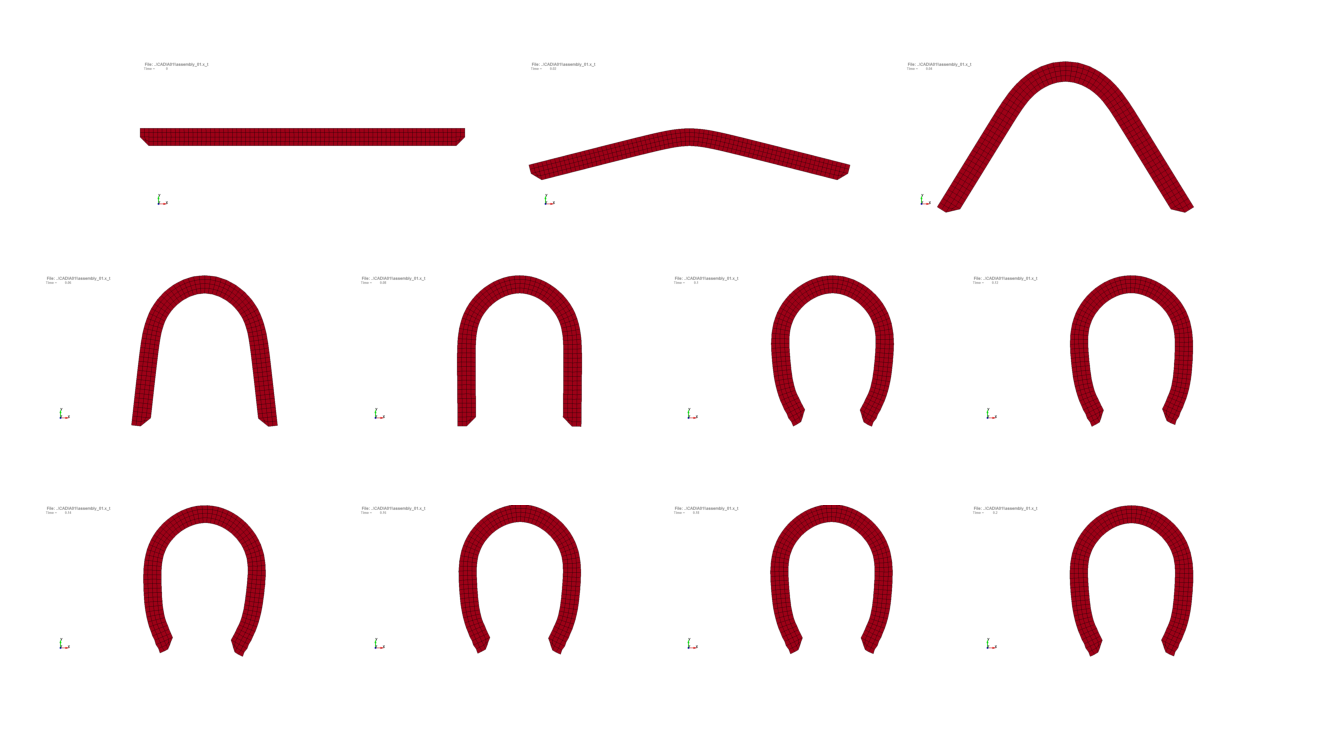
\includegraphics[width=0.95\textwidth]{src/ch4/shape_sequence_01.pdf}
% \captionof{figure}{Secuencia de la geometría resultante}
% \label{fig:shape_sequence_01}
% \end{center}

Las figuras \ref{fig:geometry_01} y \ref{fig:geometry_02} muestran las geometrías 
resultantes al final del primer y segundo paso del proceso de formado. Las formas 
obtenidas corresponden a lo esperado cuando se diseñó el herramental, y no se observan 
algún tipo de anormalidad en las geometrías obtenidas.

\begin{center}
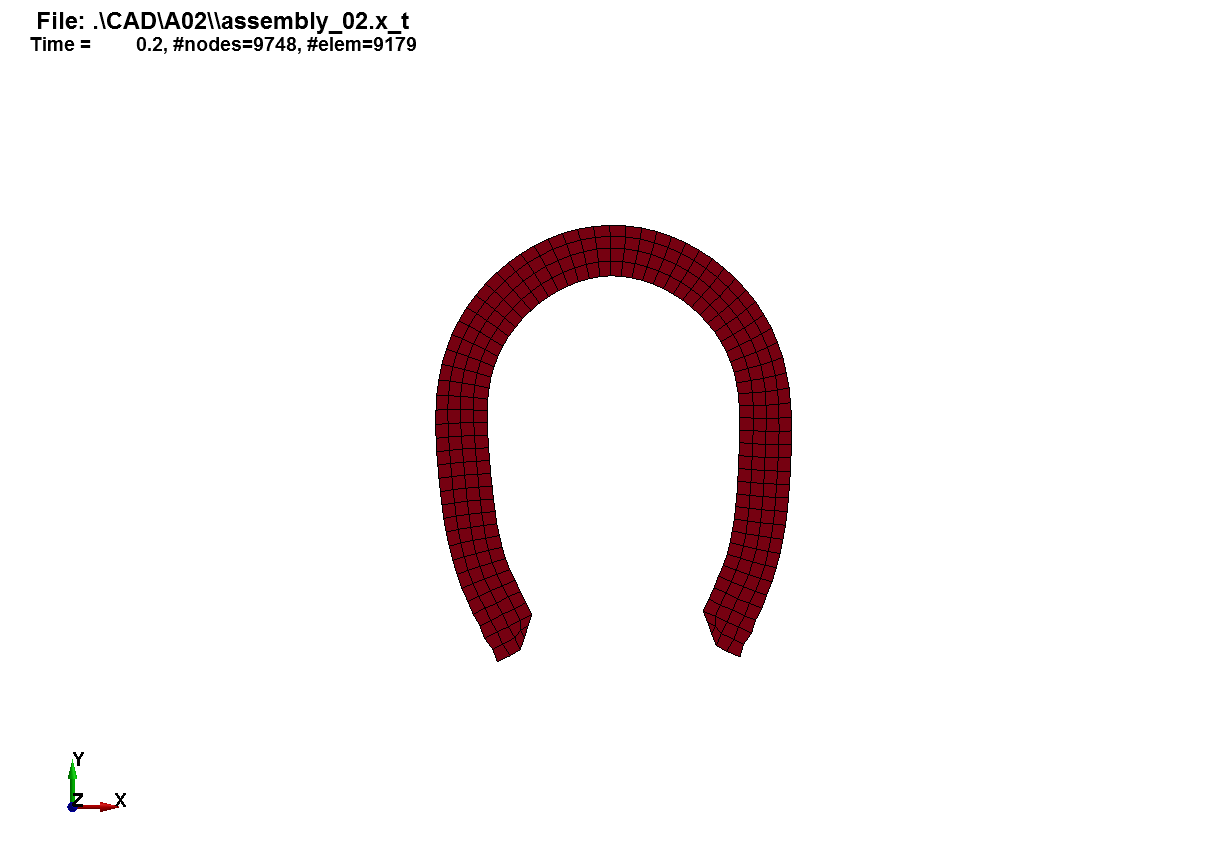
\includegraphics[width=0.75\textwidth]{src/ch4/geometry_01.png}
\captionof{figure}{Geometría resultante, primer paso}
\label{fig:geometry_01}
\end{center}

\begin{center}
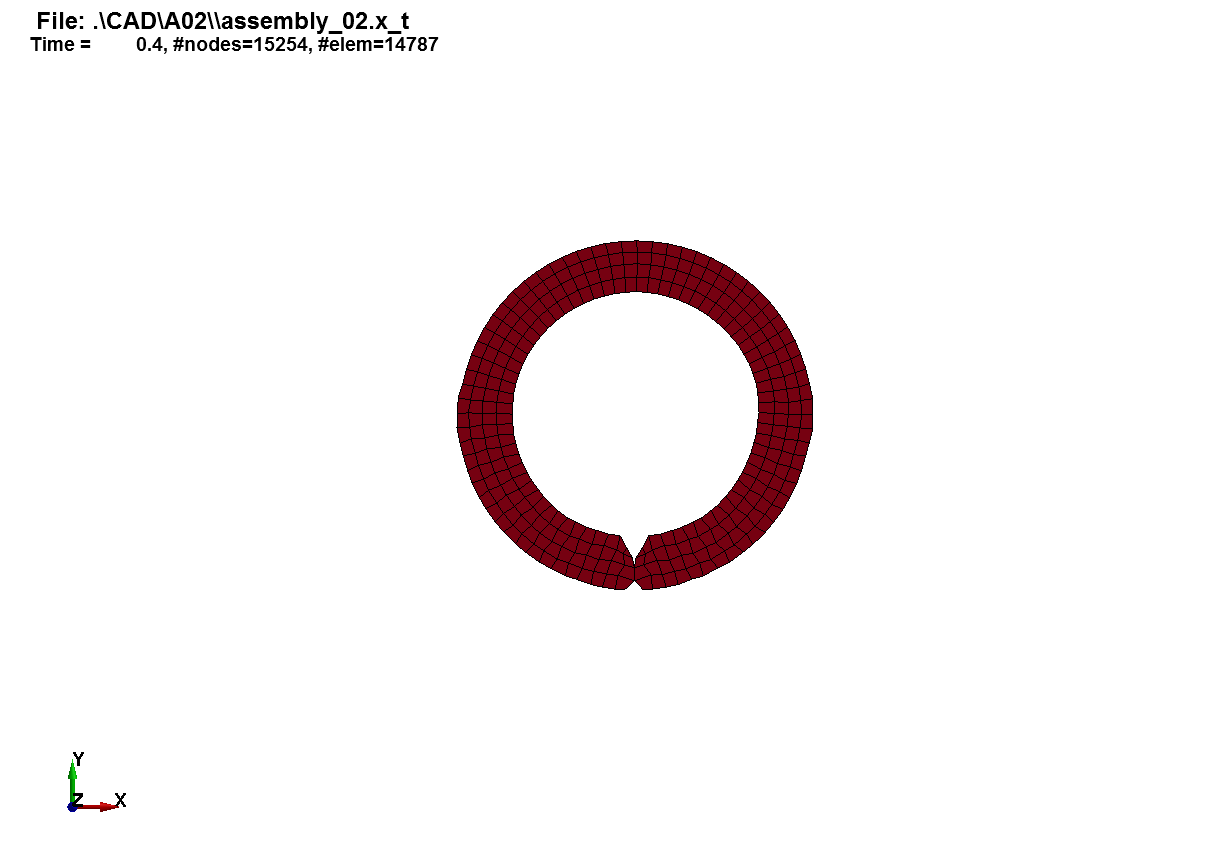
\includegraphics[width=0.75\textwidth]{src/ch4/geometry_02.png}
\captionof{figure}{Geometría resultante, segundo paso}
\label{fig:geometry_02}
\end{center}

La figura \ref{fig:thickness_variation} muestra una gráfica con las variaciones de espesor en la geometría 
final obtenida, las líneas punteadas corresponden a las tolerancias mínima y máxima del espesor. Para 
efectuar tal medición se tomaron como referencia nodos interiores y exteriores en la geometría final, 
posicionados sobre la misma vertical en la geometría inicial, y enseguida, basándose en las coordenadas 
iniciales y los desplazamientos, se obtuvo la distancia.

\begin{center}
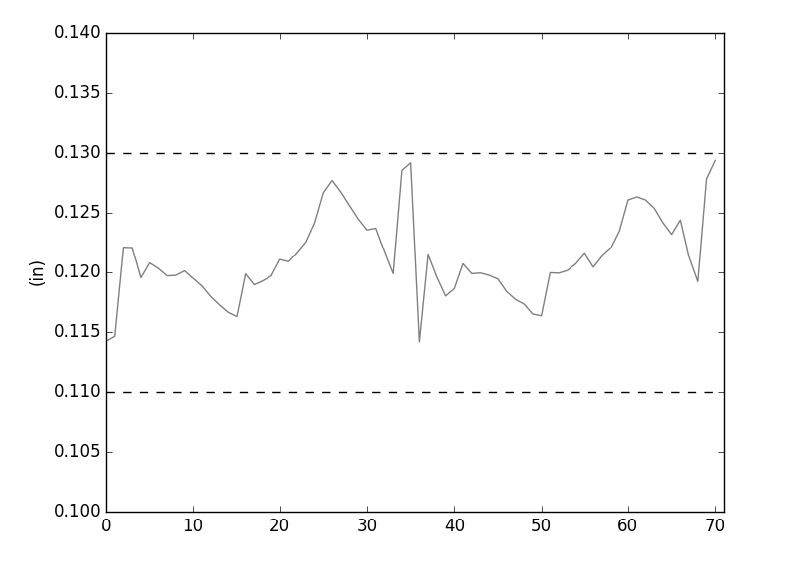
\includegraphics[width=0.75\textwidth]{src/ch4/thickness_variation.png}
\captionof{figure}{Variación del espesor de la geometría resultante}
\label{fig:thickness_variation}
\end{center}

\subsubsection{Esfuerzos}

\begin{center}
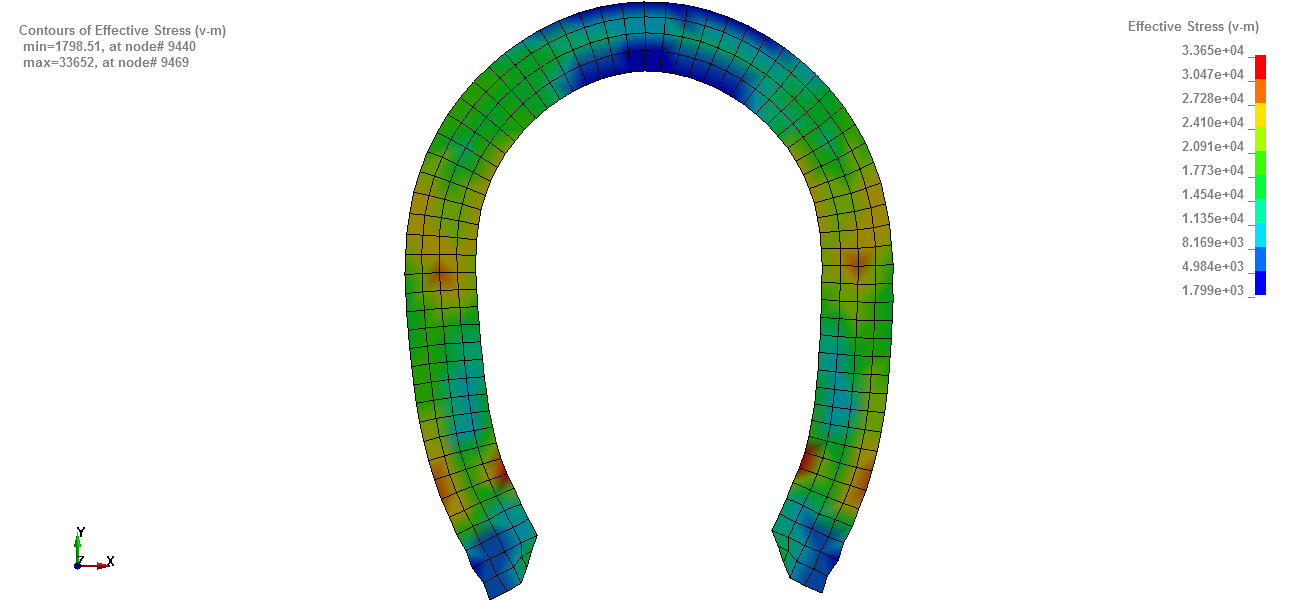
\includegraphics[width=0.75\textwidth]{src/ch4/von_mises_01.png}
\captionof{figure}{Distribución de esfuerzos de von Mises, final del primer paso}
\label{fig:von_mises_01}
\end{center}

\begin{center}
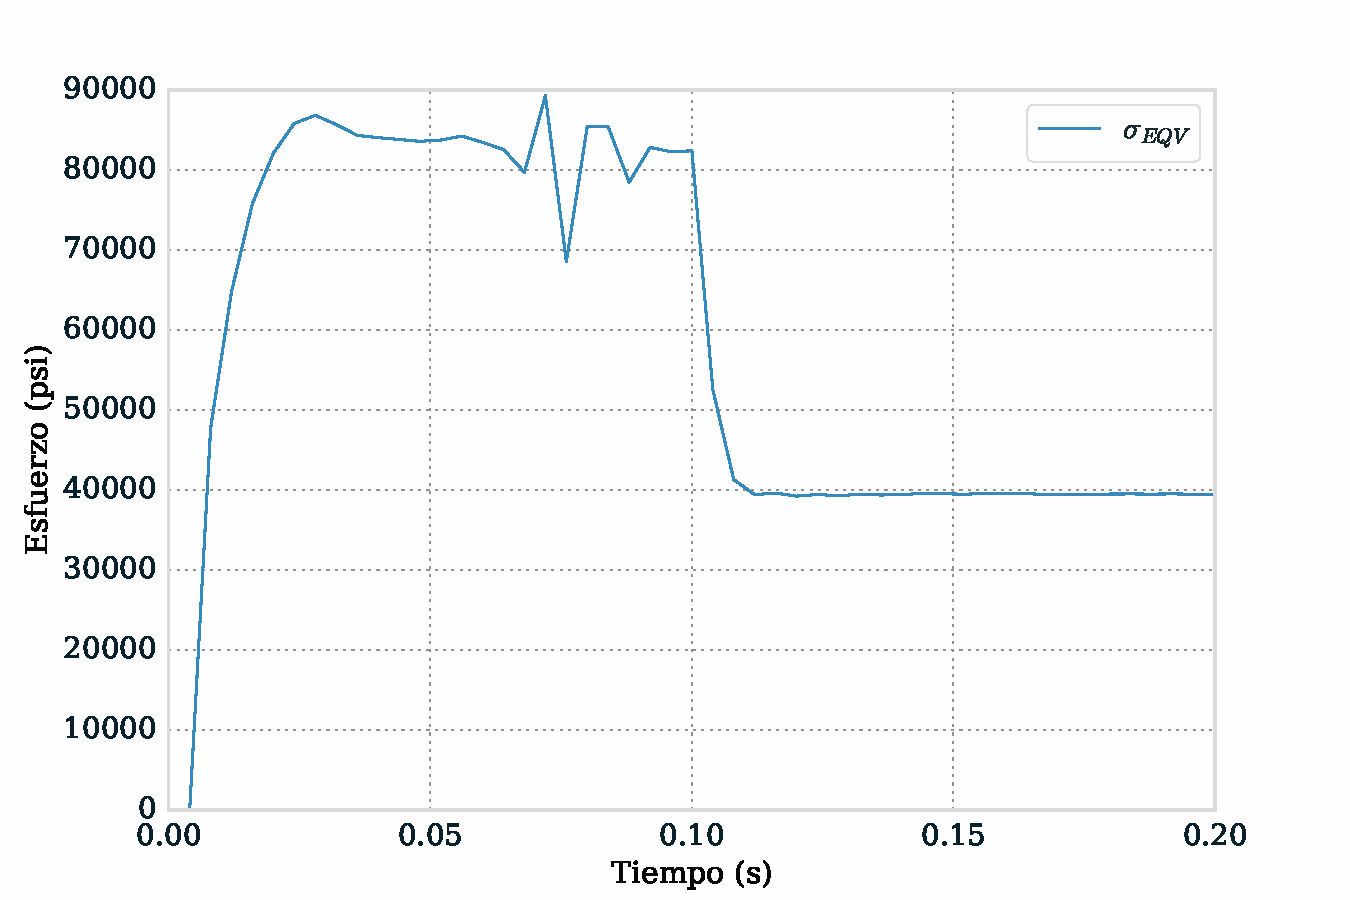
\includegraphics[width=0.75\textwidth]{src/ch4/von_mises_stress_01.pdf}
\captionof{figure}{Variación del esfuerzo máximo de von Mises}
\label{fig:von_mises_stress_01}
\end{center}

\begin{center}
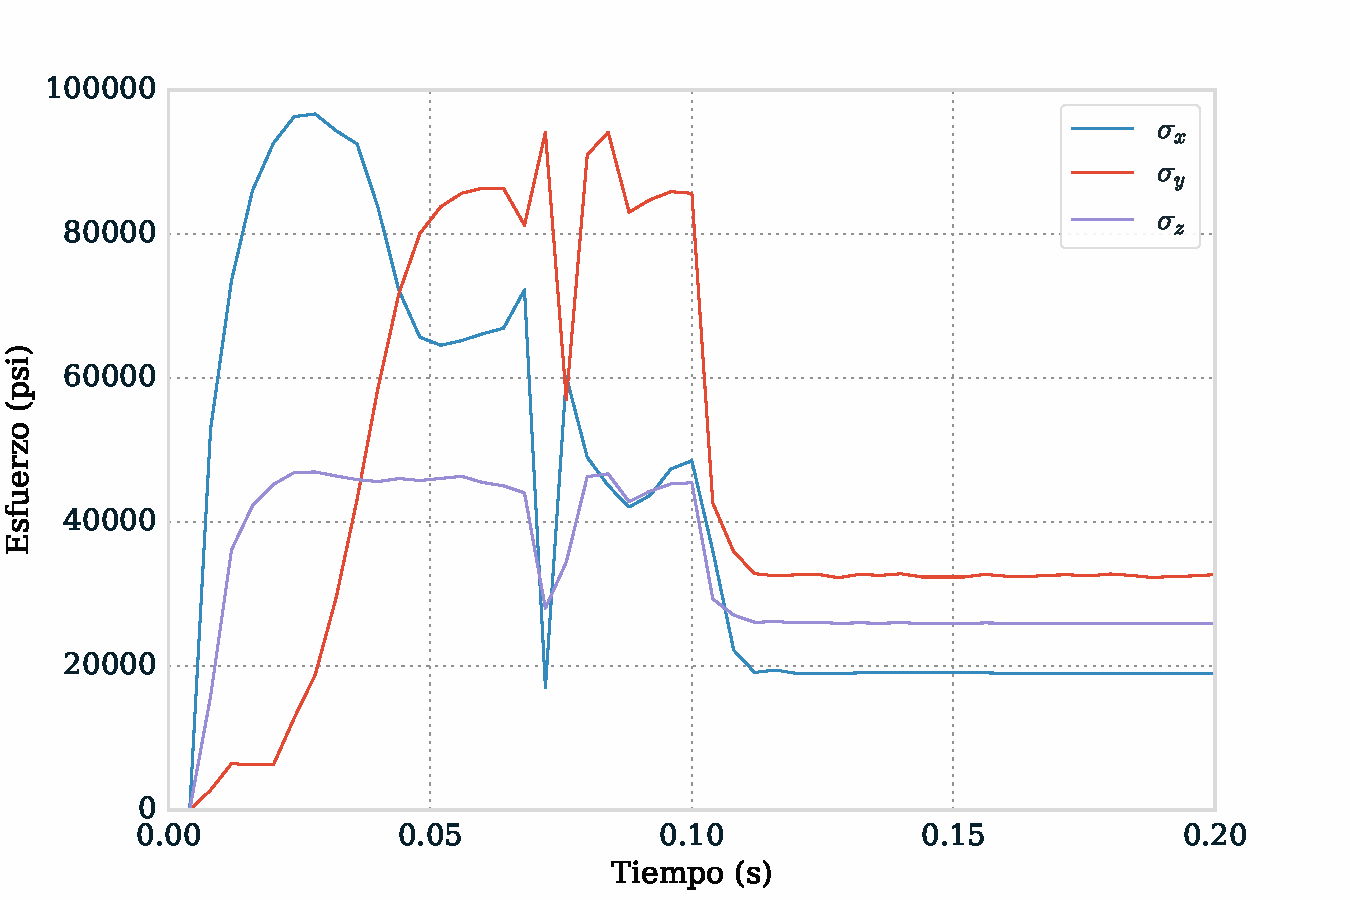
\includegraphics[width=0.75\textwidth]{src/ch4/xyz_stress_01.pdf}
\captionof{figure}{Variación de los esfuerzos máximos en dirección X,Y,Z}
\label{fig:xyz_stress_01}
\end{center}

\begin{center}
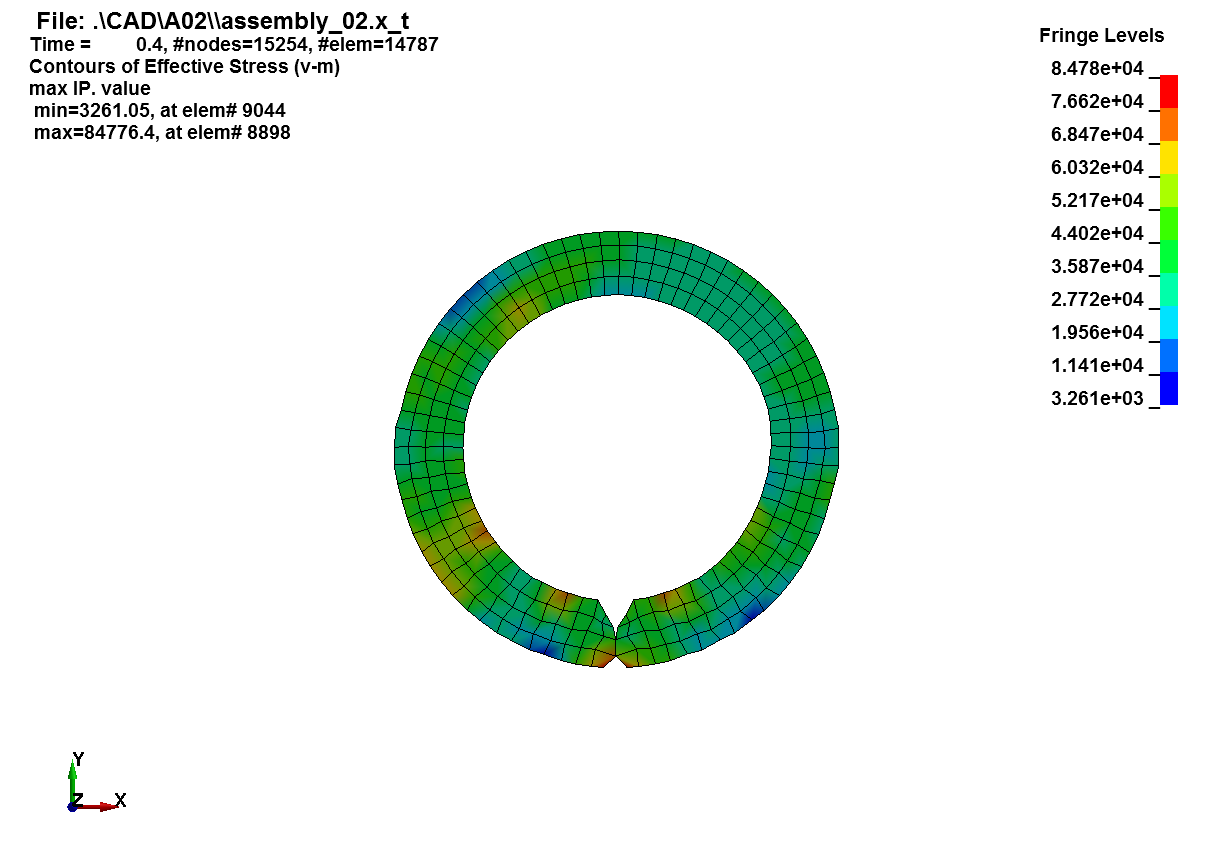
\includegraphics[width=0.75\textwidth]{src/ch4/von_mises_02.png}
\captionof{figure}{Distribución de esfuerzos de von Mises, final del segundo paso}
\label{fig:von_mises_01}
\end{center}


\subsubsection{Deformaciones}

\begin{center}
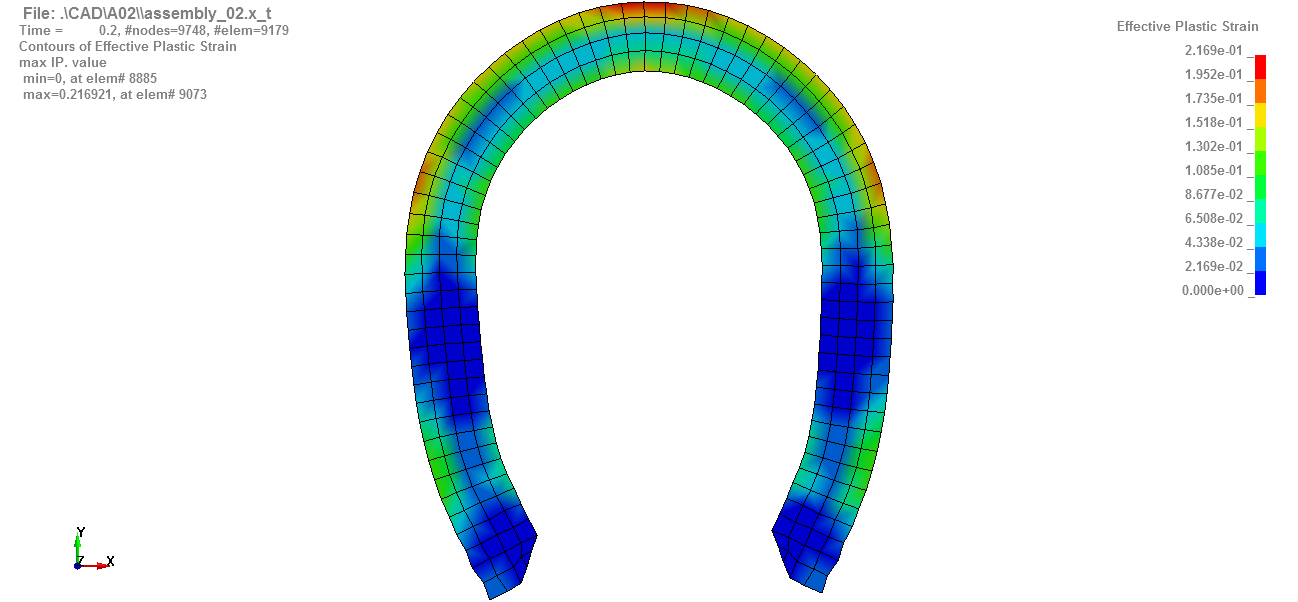
\includegraphics[width=0.75\textwidth]{src/ch4/efective_plastic_strain_01.png}
\captionof{figure}{Deformación plástica efectiva, final del primer paso}
\label{fig:efective_plastic_strain}
\end{center}

% \begin{center}
% 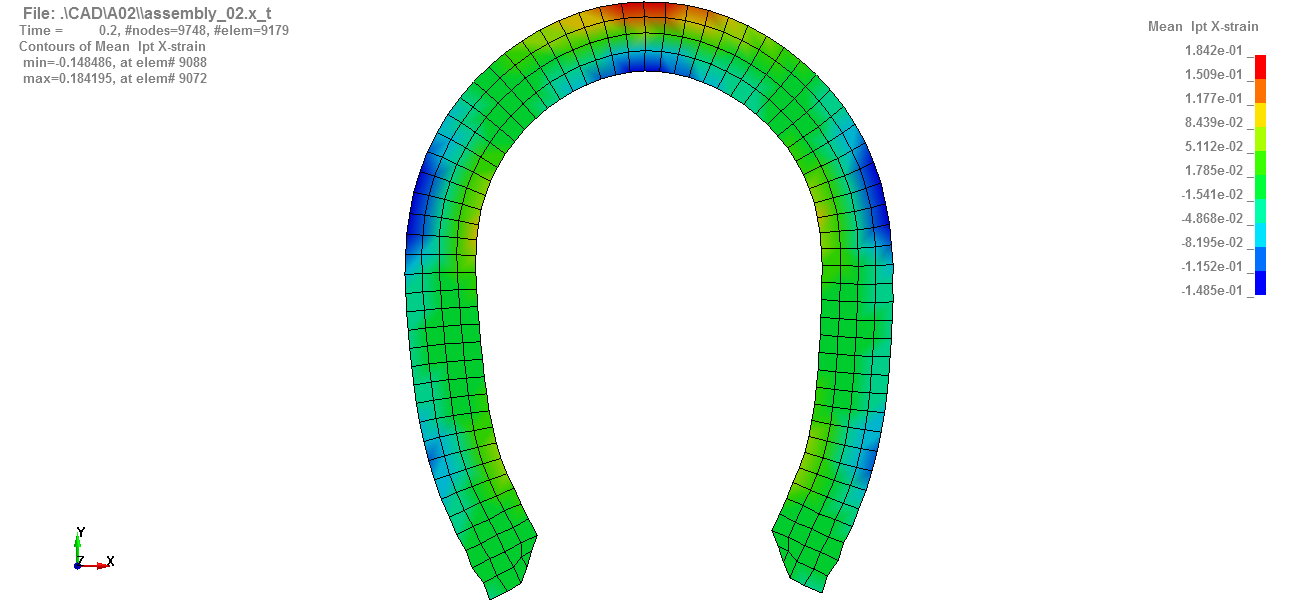
\includegraphics[width=0.75\textwidth]{src/ch4/strain_x_01.png}
% \captionof{figure}{Deformación en dirección X, final del primer paso}
% \label{fig:efective_plastic_strain}
% \end{center}

% \begin{center}
% 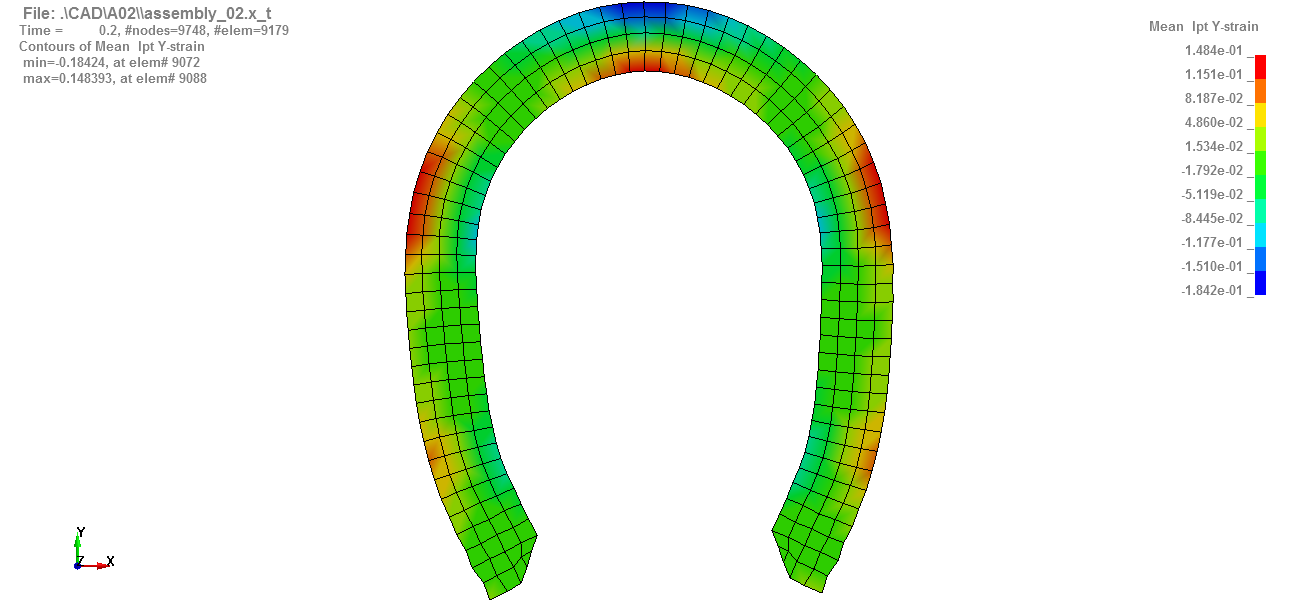
\includegraphics[width=0.75\textwidth]{src/ch4/strain_y_01.png}
% \captionof{figure}{Deformación en dirección Y, final del primer paso}
% \label{fig:efective_plastic_strain}
% \end{center}


\begin{center}
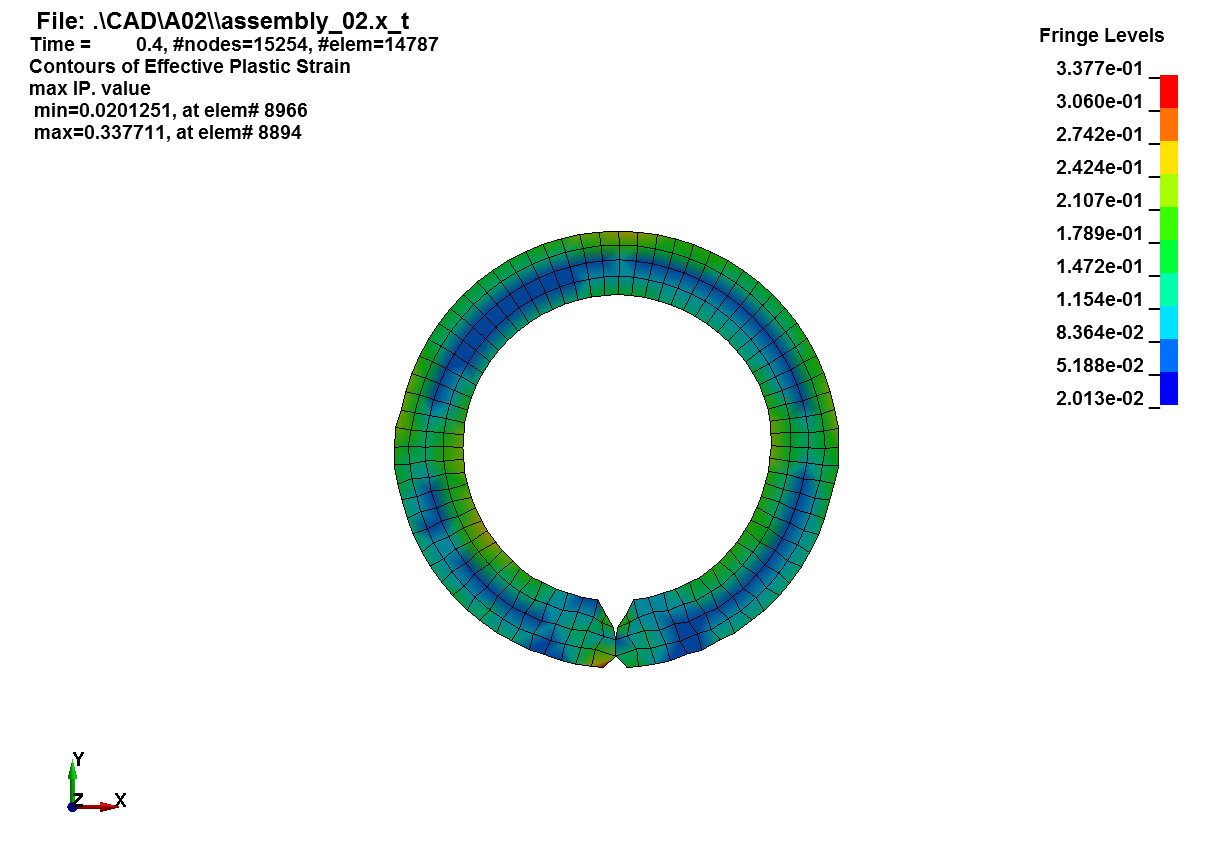
\includegraphics[width=0.75\textwidth]{src/ch4/efective_plastic_strain_02.png}
\captionof{figure}{Deformación plástica efectiva, final del segundo paso}
\label{fig:efective_plastic_strain}
\end{center}

% \begin{center}
% 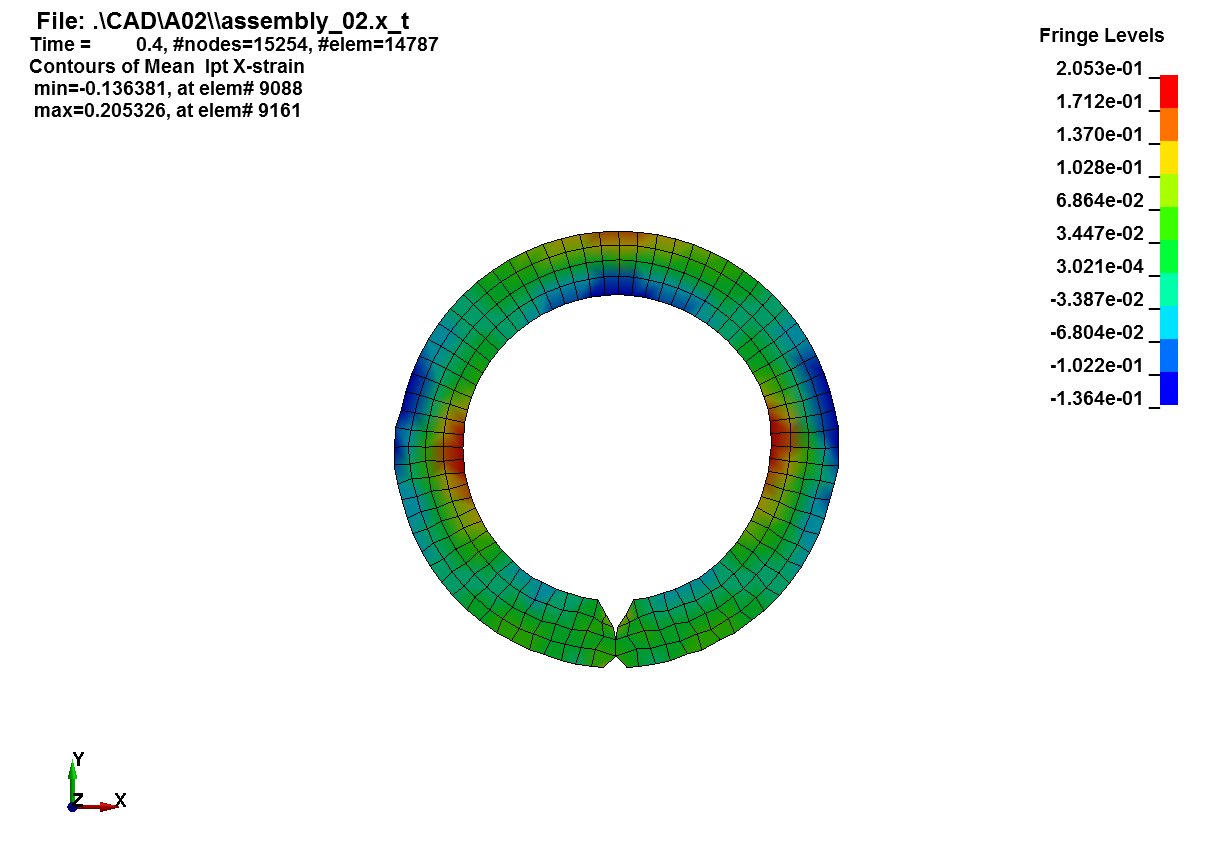
\includegraphics[width=0.75\textwidth]{src/ch4/strain_x_02.png}
% \captionof{figure}{Deformación en dirección X, final del segundo paso}
% \label{fig:efective_plastic_strain}
% \end{center}

% \begin{center}
% 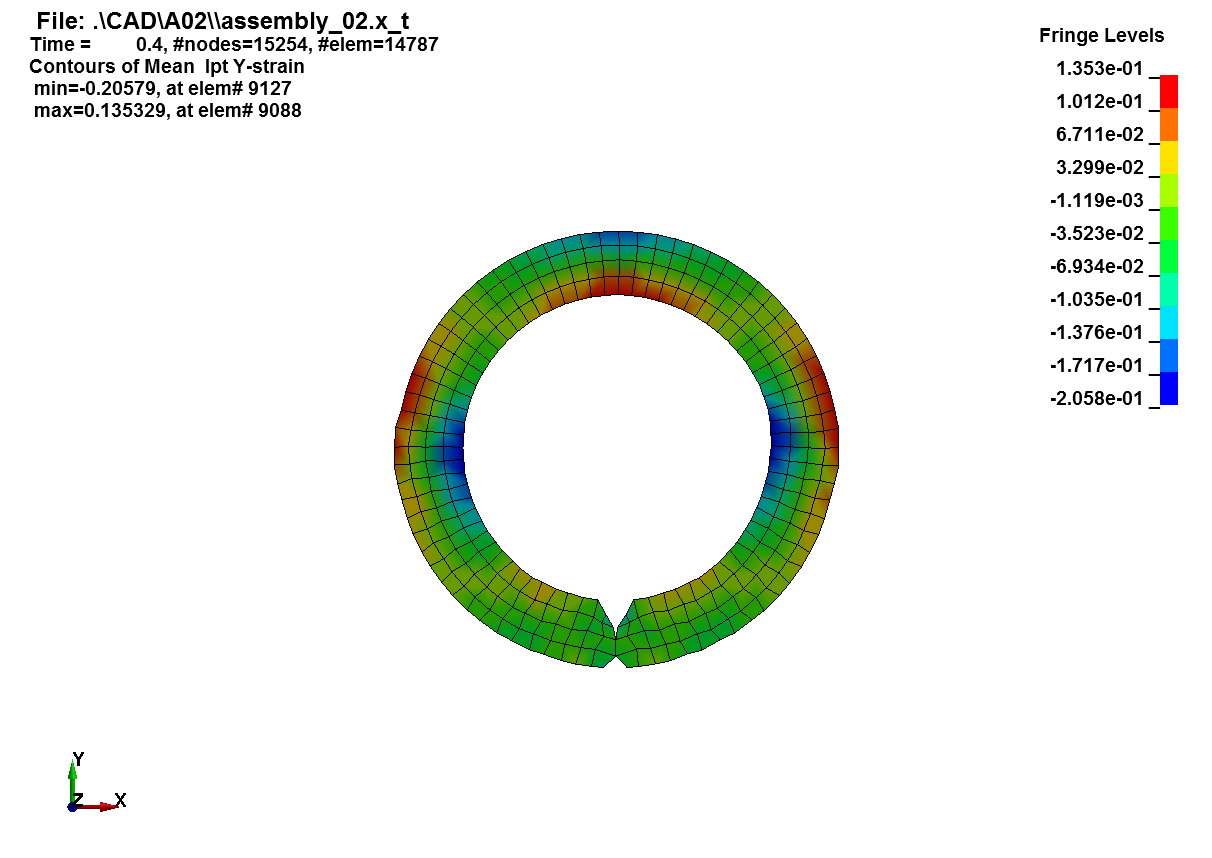
\includegraphics[width=0.75\textwidth]{src/ch4/strain_y_02.png}
% \captionof{figure}{Deformación en dirección Y, final del segundo paso}
% \label{fig:efective_plastic_strain}
% \end{center}


\subsubsection{Fuerza de formado}

\begin{center}
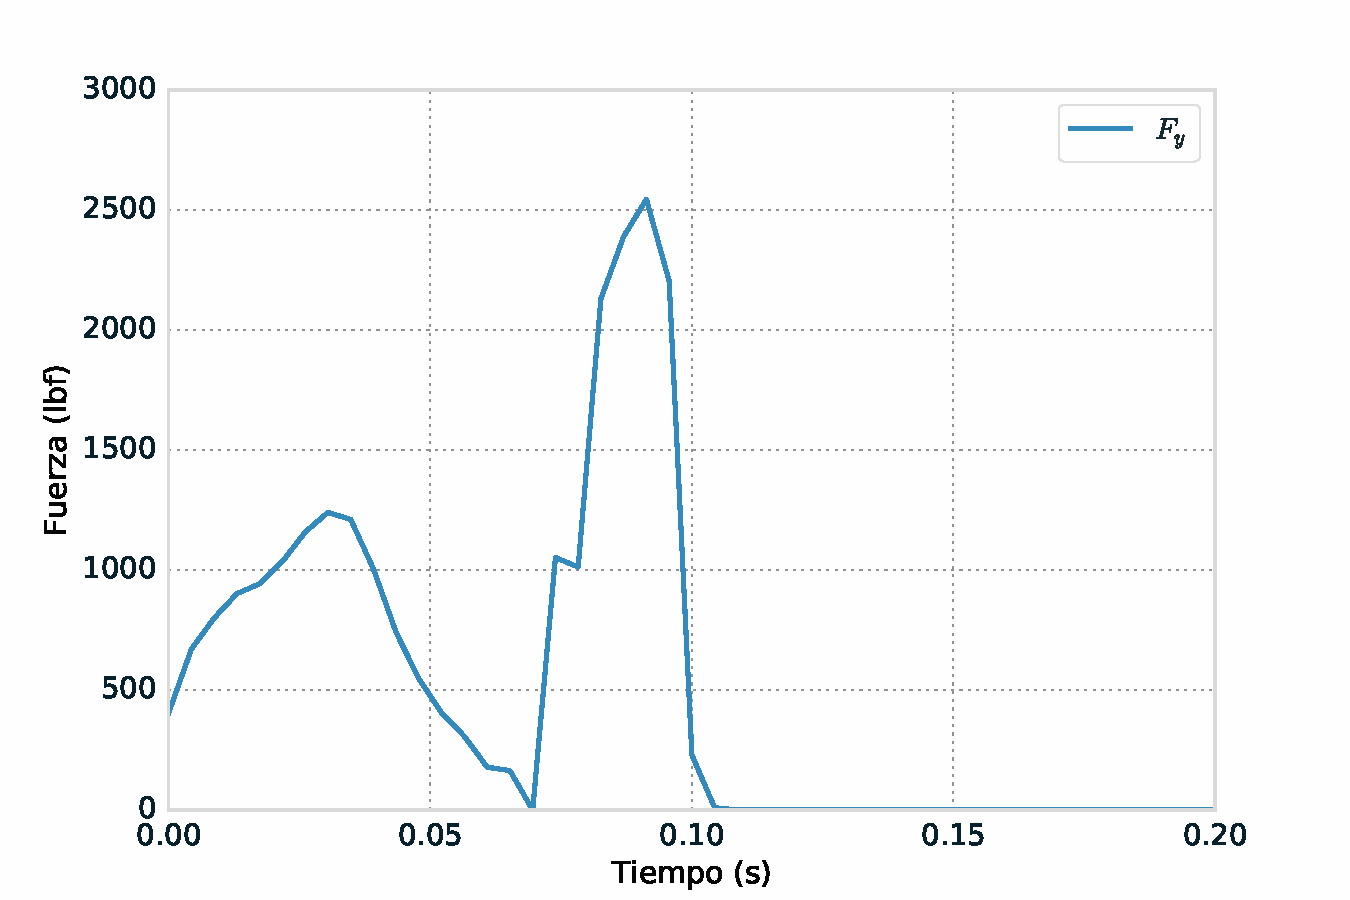
\includegraphics[width=0.75\textwidth]{src/ch4/nodal_force_01.pdf}
\captionof{figure}{Fuerza de formado requerida, primer paso}
\label{fig:nodal_force_01}
\end{center}


\subsubsection{Influencia del escalamiento de masa}

En la sección \ref{sec:mass-scaling} se describió el proceso para utilizar el escalamiento de masa 
selectivo en un análisis de tipo dinámico explícito, cuyo objetivo es reducir el tiempo de 
solución de una simulación mediante la introducción controlada de \textit{masa artificial} que implica 
un aumento en la densidad del material y esto a su vez la reducción de los intervalos de tiempo.\\

En lo subsiguiente se presenta el análisis de cinco simulaciones realizadas con escalamientos de 
masa selectivo, en donde el tamaño mínimo del paso de tiempo se varía desde $1x10^{-7}$ hasta 
$5x10^{-7}$.\\

La figura \ref{fig:ms_sol_time} muestra la variación del tiempo de solución (CPU Time) comparado con 
el porcentaje de masa agregado. Se observa que la curva resultante muestra el comportamiento de 
una función exponencial decreciente y que con un 12\% de masa adicional se puede reducir el tiempo 
de solución hasta un 30\% respecto al tiempo de solución sin escalamiento de masa.

\begin{center}
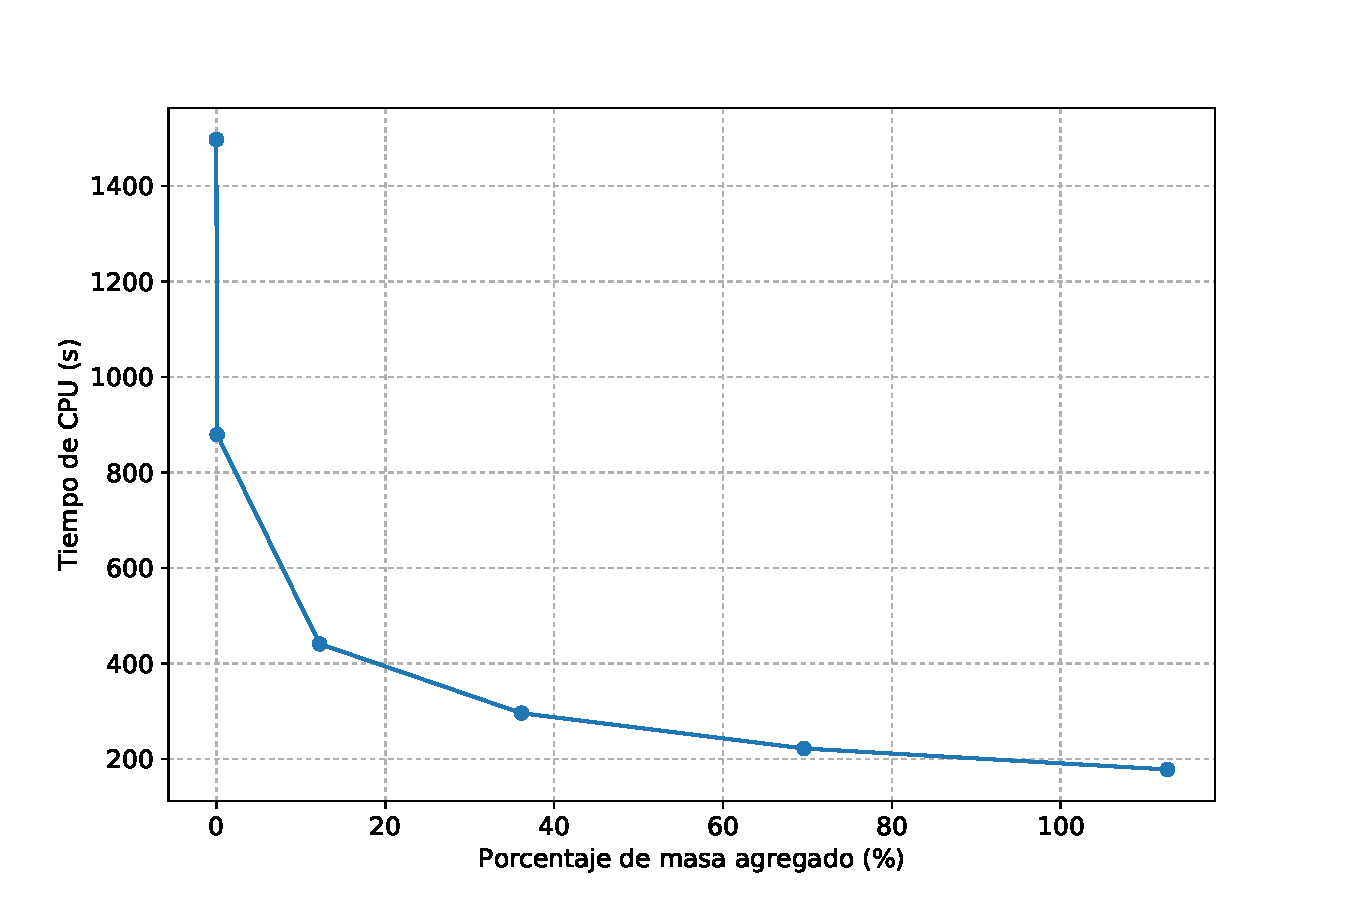
\includegraphics[width=0.75\textwidth]{src/ch4/ms_sol_time.pdf}
\captionof{figure}{Tiempo de solución para diversos escalamientos de masa}
\label{fig:ms_sol_time}
\end{center}

En \ref{fig:ms_von_mises} se muestra la variación del esfuerzo equivalente máximo de von Mises, cuando 
se aplica el escalamiento de masa. Se puede observar que la variación entre cada uno de los casos 
es mínima en todo el hsitorial de tiempo, habiendo una diferencia significativa en el tiempo 
correspondiente a cuando los formadores superiores dejan de actuar y las levas aún no interactúan 
con la pieza de trabajo.

\begin{center}
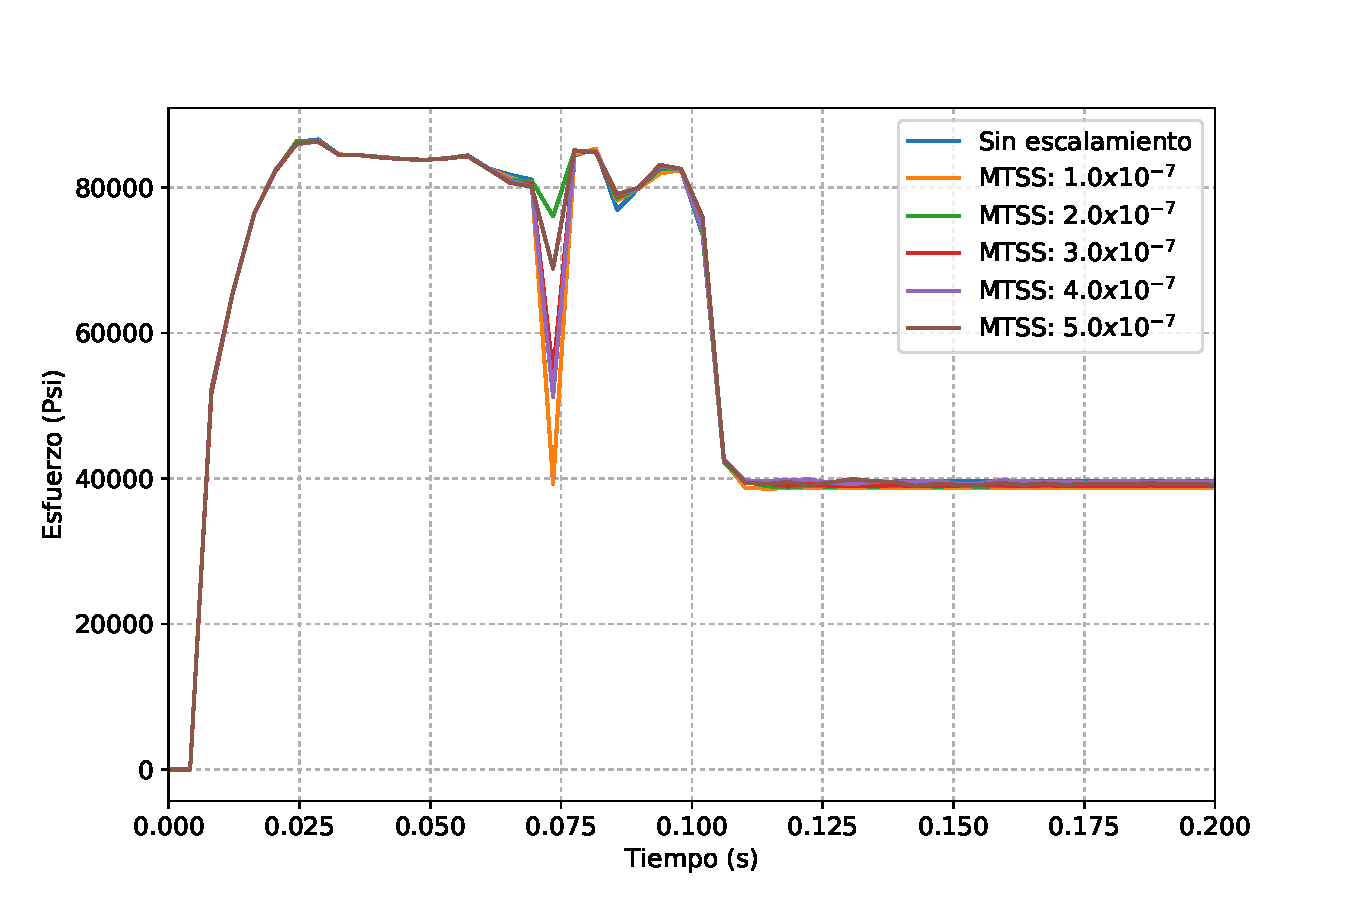
\includegraphics[width=0.75\textwidth]{src/ch4/ms_von_mises.pdf}
\captionof{figure}{Variación del esfuerzo de von Mises utilizando escalamiento de masa}
\label{fig:ms_von_mises}
\end{center}

En \ref{fig:ms_force} se muestra la variación de la fuerza de formado, se observa que el 
comportamiento es prácticamente similar para todos los casos.

\begin{center}
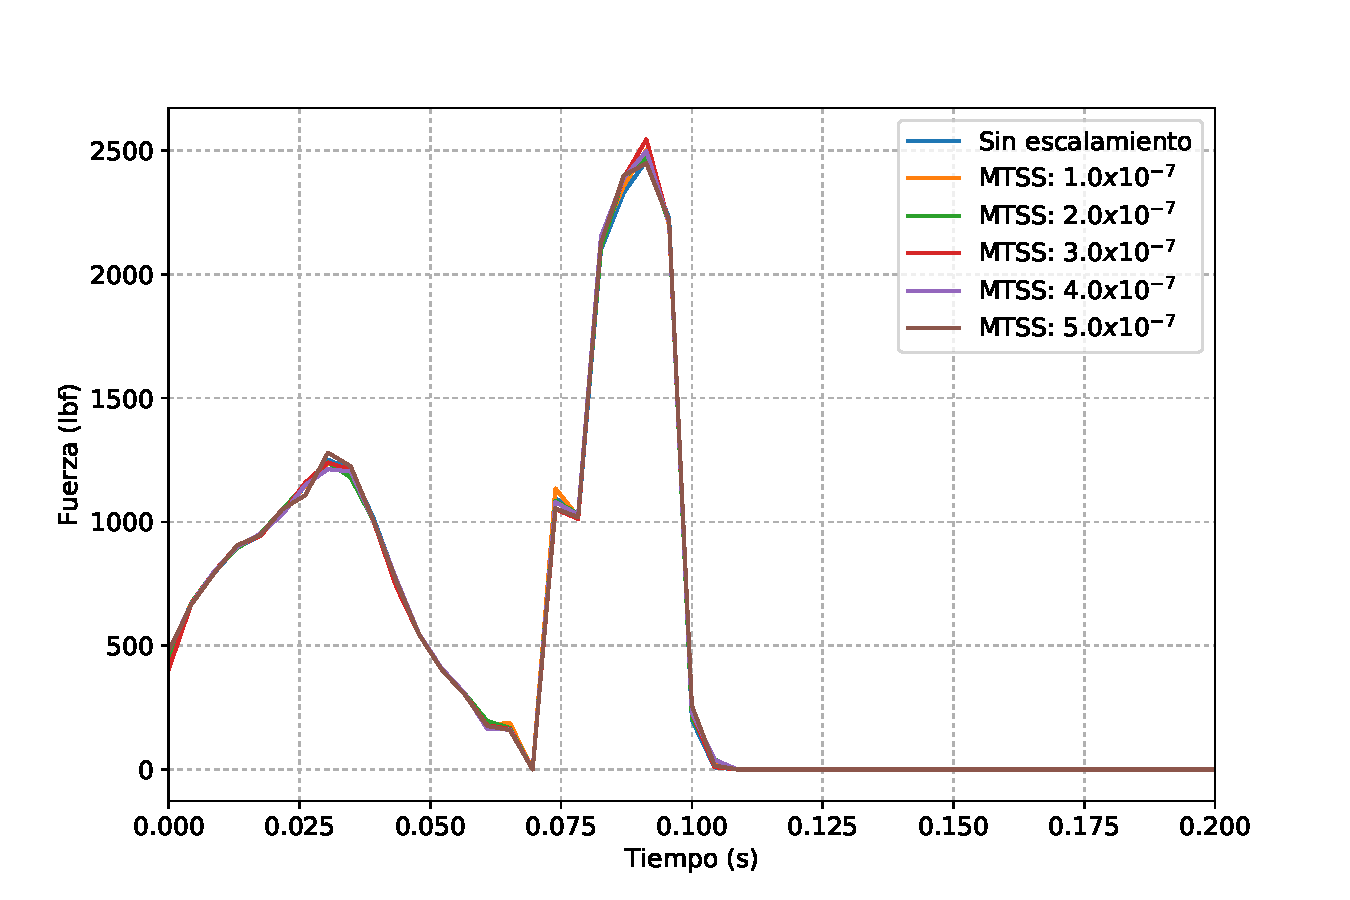
\includegraphics[width=0.75\textwidth]{src/ch4/ms_force.pdf}
\captionof{figure}{Variación de la fuerza de formado usando escalamiento de masa}
\label{fig:ms_force}
\end{center}

Con lo observado, se puede asumir que la influencia del escalamiento de masa, agregando hasta alrededor 
de un 110\% de masa, no es significativa, y permite reducir hasta en un 90\% el tiempo de solución de 
un análisis dinámico-explícito, lo cual representa una enorme ventaja.

\subsubsection{Modelos de material}

En las figuras  \ref{fig:mdm_von_mises} y \ref{fig:mdm_force} se muestran las gráficas correspondientes 
al esfuerzo máximo de von Mises y la fuerza de formado, respectivamente, de la evaluación de los diversos 
modelos de material que ahí se listan.\\

Tanto la variación de los esfuerzos, como la de la fuerza de formado, es poco significativa, mostrando 
un comportamiento similar en ambos casos para todos los modelos de material utilizados. La 
diferencia más notoria ocurre en los esfuerzos residuales que quedan al finalizar el proceso 
de formado, en donde se observa una diferencia de alrededor de un 20\% del modelo multilineal 
respecto al bilineal cinemático.

\begin{center}
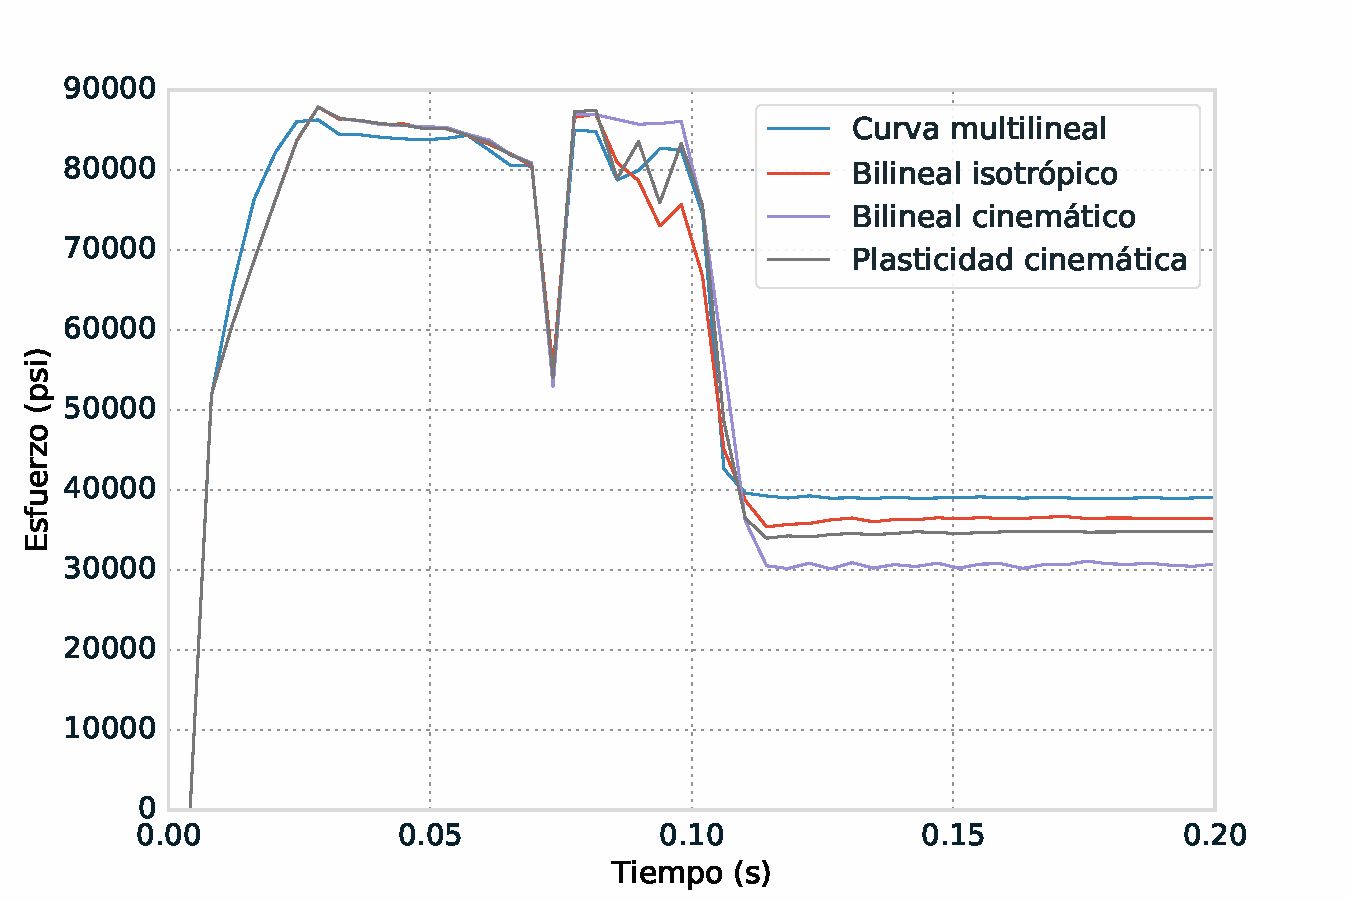
\includegraphics[width=0.75\textwidth]{src/ch4/mdm_von_mises.pdf}
\captionof{figure}{Variación de la fuerza de formado usando escalamiento de masa}
\label{fig:mdm_von_mises}
\end{center}

\begin{center}
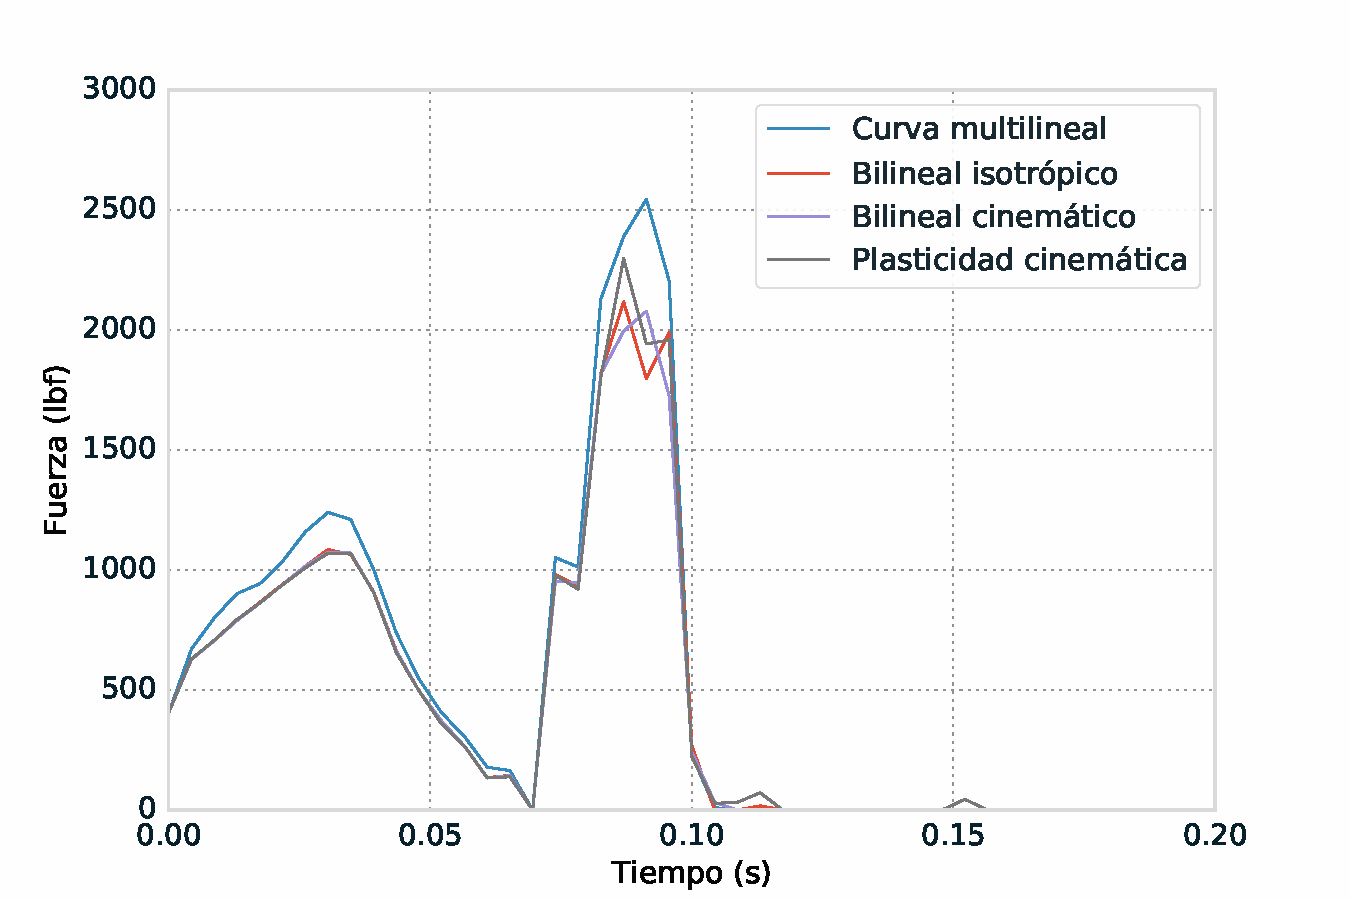
\includegraphics[width=0.75\textwidth]{src/ch4/mdm_force.pdf}
\captionof{figure}{Variación de la fuerza de formado usando escalamiento de masa}
\label{fig:mdm_force}
\end{center}

\subsection{Análisis 3D}


% \subsubsection{Estatus global}

% \begin{center}
% 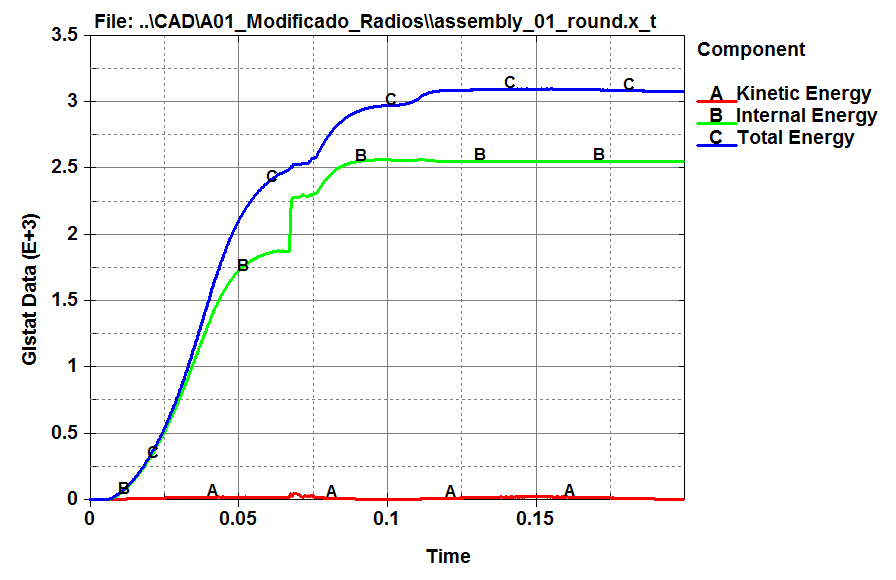
\includegraphics[width=0.75\textwidth]{src/ch4/energy_status_3d.png}
% \captionof{figure}{Energía interna, cinética y total}
% \label{fig:von_mises_3D_01}
% \end{center}

\subsubsection{Esfuerzos}


\begin{center}
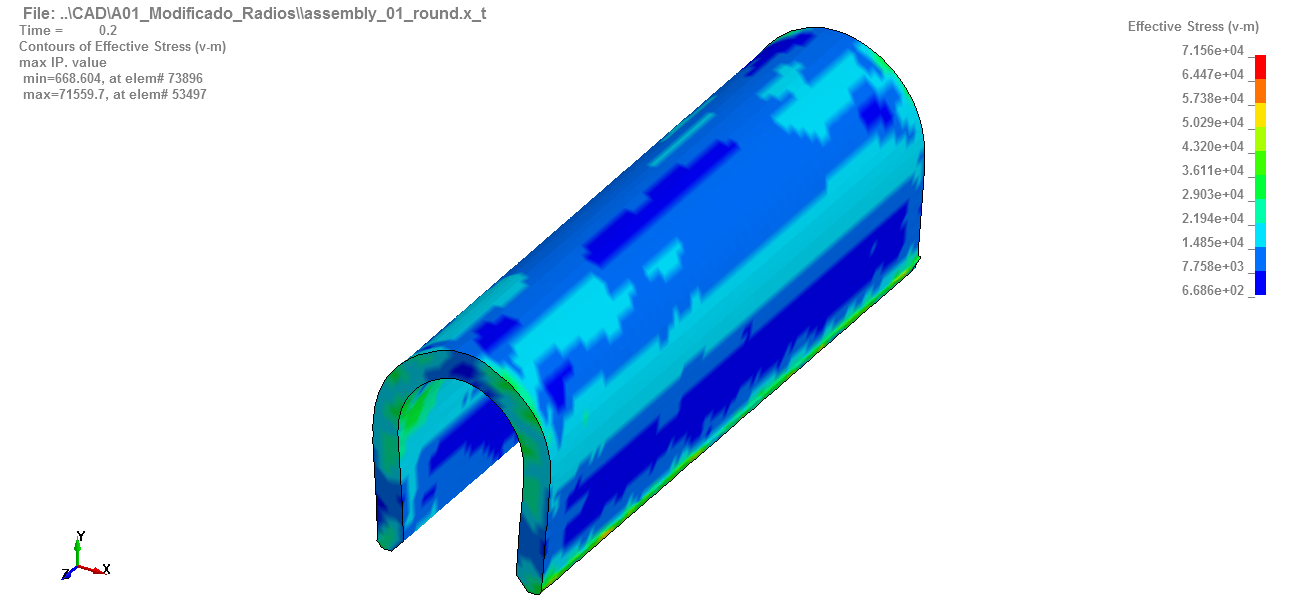
\includegraphics[width=0.75\textwidth]{src/ch4/von_mises_3D_01.png}
\captionof{figure}{Distribución del esfuerzo de von Mises}
\label{fig:von_mises_3D_01}
\end{center}

\begin{center}
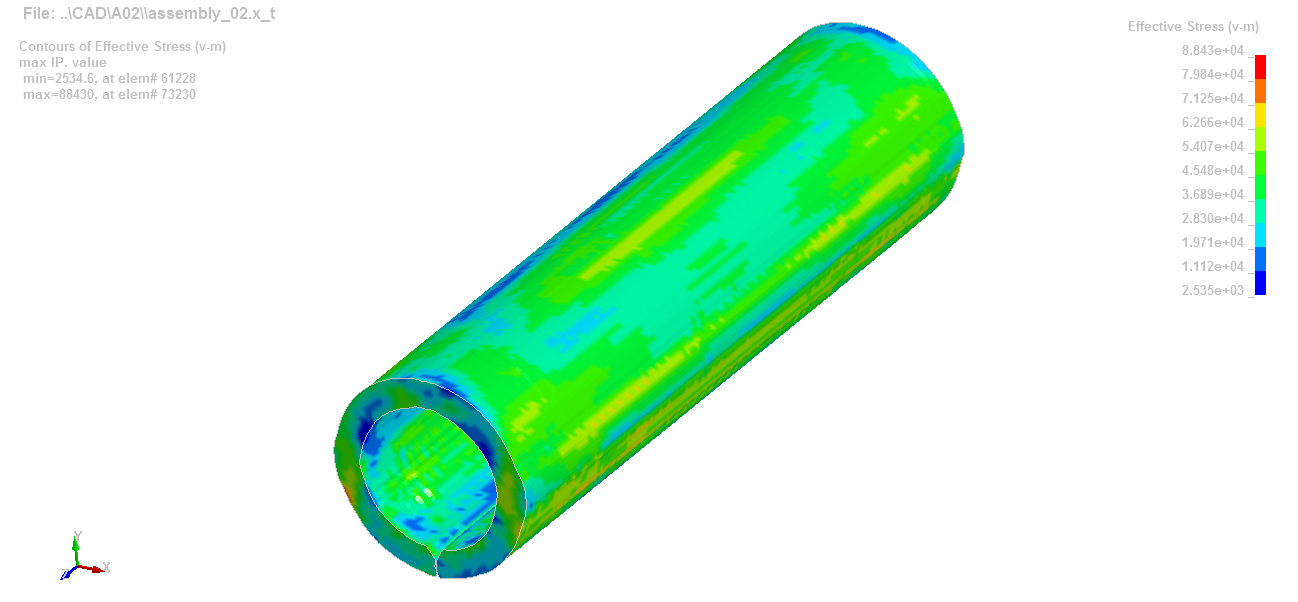
\includegraphics[width=0.75\textwidth]{src/ch4/von_mises_3D_02.png}
\captionof{figure}{Distribución del esfuerzo de von Mises, segundo paso}
\label{fig:von_mises_3D_02}
\end{center}

\subsubsection{Deformaciones}

\begin{center}
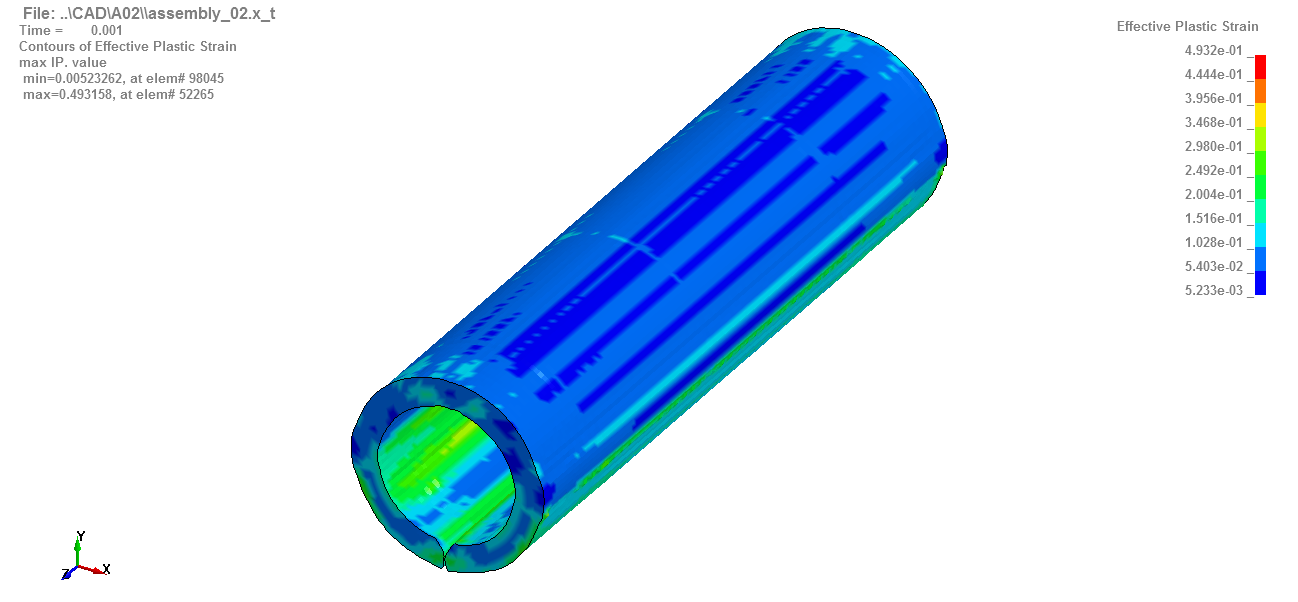
\includegraphics[width=0.75\textwidth]{src/ch4/eqv_strain_01.png}
\captionof{figure}{Deformación plástica equivalente, primer paso}
\label{fig:eqv_strain_01}
\end{center}


\subsection{Comparación 2D vs 3D}

En esta sección se presenta un análisis comparativo entre el análisis bidimensional 
y el análisis en tres dimensiones.

\subsubsection{Tiempo de cómputo}

\subsubsection{Fuerza de formado}


\section{Del análisis experimental}


